%
% \iffalse
%
%% drivers.dtx Copyright (C) 1994      David Carlisle Sebastian Rahtz
%%             Copyright (C) 1995 1996 1997 1998 1999 David Carlisle
%%             Copyright (C) 2000-2020 David Carlisle, LaTeX3 Project
%%
%% This file is part of the Standard LaTeX `Graphics Bundle'.
%% It may be distributed under the terms of the LaTeX Project Public
%% License, as described in lppl.txt in the base LaTeX distribution.
%% Either version 1.3 or, at your option, any later version.
%%
%<template, >\ProvidesFile{template.def}
%<dvips,    >\ProvidesFile{dvips.def}
%<dvipsnames>\ProvidesFile{dvipsnam.def}
%<dvipdf,   >\ProvidesFile{dvipdf.def}
%<emtex,    >\ProvidesFile{emtex.def}
%<dviwin,   >\ProvidesFile{dviwin.def}
%<dvipsone, >\ProvidesFile{dvipsone.def}
%<pctexps,  >\ProvidesFile{pctexps.def}
%<pctex32,  >\ProvidesFile{pctex32.def}
%<pctexwin, >\ProvidesFile{pctexwin.def}
%<pctexhp,  >\ProvidesFile{pctexhp.def}
%<truetex,  >\ProvidesFile{truetex.def}
%<tcidvi,   >\ProvidesFile{tcidvi.def}
%<oztex,    >\ProvidesFile{oztex.def}
%<textures, >\ProvidesFile{textures.def}
%<dvialw,   >\ProvidesFile{dvialw.def}
%<dvilaser, >\ProvidesFile{dvilaser.def}
%<psprint,  >\ProvidesFile{psprint.def}
%<dvi2ps,   >\ProvidesFile{dvi2ps.def}
%<pubps,    >\ProvidesFile{pubps.def}
%<dvitops,  >\ProvidesFile{dvitops.def}
%<ln,       >\ProvidesFile{ln.def}
%
%<*driver>
    \NeedsTeXFormat{LaTeX2e}
    \ProvidesFile{drivers.dtx}
%</driver>
        [2016/06/17 v3.0m Driver-dependent file (DPC,SPQR)]
%
%<*driver>
    \documentclass{ltxdoc}
    \GetFileInfo{drivers.dtx}
 \begin{document}
   \title{Graphics drivers for \LaTeXe\thanks
     {Version \fileversion, revised \filedate}}
   \author{Sebastian Rahtz and David Carlisle}
   \date{\filedate}
   \MaintainedByLaTeXTeam{graphics}
   \maketitle
   \DocInput{drivers.dtx}
 \end{document}
%</driver>
% \fi
%
%
%
% \providecommand\OzTeX{O\kern-.03em z\kern-.15em\TeX}
%
% \section{Driver files}
%
% This file implements some of the currently supported drivers.
% If the driver you use is not in this list then a `.def' file
% may be distributed with This graphics bundle,
% or may be distributed with your driver.
%
% If not, send us some details of the driver's |\special| syntax, and
% we will try to produce a suitable file.
%
% Note that some of these files are for drivers to which we have no
% access, so they are untested. Please send any corrections to the
% latexbugs address.
%
%
%
%
% \StopEventually{}
%
%
% \section{Colour}
%
% Most of the drivers that support colour use one of three methods.
% \begin{itemize}
% \item color1: `dvips' style colour specials.
% \item color2: `textures' style colour specials.
% \item color3: Colour implemented via literal PostScript specials.
% \item color4: Colour implemented by specials that only support RGB,
%               i.e., Red Green Blue specified as integers in the range
%               0--255. Other models converted to this within \TeX.
% \end{itemize}
% Some drivers do not use any of these modules and have their own code.
% Note that drivers using the `color3' code can not fully support the
% \LaTeX\ colour commands.
%    \begin{macrocode}
%<*color1|color2|color3|color4>
%    \end{macrocode}
%
%    \begin{macrocode}
\def\c@lor@arg#1{%
  \dimen@#1\p@
  \ifdim\dimen@<\z@\dimen@\maxdimen\fi
  \ifdim\dimen@>\p@
    \PackageError{color}{Argument `#1' not in range [0,1]}\@ehd
  \fi}
%    \end{macrocode}
%
% Need to make sure of a trailing .0 for textures. Apparently it
% is OK to always add a . as 1.3. is accepted by textures.
% textures gray special is reversed, so just use rgb instead.
%
%    \begin{macrocode}
\def\color@gray#1#2{%
  \c@lor@arg{#2}%
%<color4>  \c@lor@rgb@RGB\@tempa
%<color1>  \edef#1{gray #2}%
%<color2>  \edef#1{rgb #2. #2. #2.}%
%<color3>  \edef#1{#2 setgray}%
%<color4>  \edef#1{\@tempa\@tempa\@tempa}%
  }
%    \end{macrocode}
%
%    \begin{macrocode}
\def\color@cmyk#1#2{\c@lor@@cmyk#2\@@#1}
\def\c@lor@@cmyk#1,#2,#3,#4\@@#5{%
  \c@lor@arg{#4}%
%<color4>    \dimen@ii#4\p@
  \c@lor@arg{#1}%
%<color4>  \c@lor@cmyk@RGB\@tempa
  \c@lor@arg{#2}%
%<color4>  \c@lor@cmyk@RGB\@tempb
  \c@lor@arg{#3}%
%<color4>  \c@lor@cmyk@RGB\@tempc
%<color1>  \edef#5{cmyk #1 #2 #3 #4}%
%<color2>  \edef#5{cmyk #1. #2. #3. #4.}%
%<color3>  \edef#5{#1 #2 #3 #4 setcmykcolor}%
%<color4>  \edef#5{\@tempa\@tempb\@tempc}%
  }
%    \end{macrocode}
%
% A 0--1 range value will have been left in |\dimen@| by |\c@lor@arg|.
% The black value (0--1) will be stored in |\dimen@ii|.
% Covert to 0--255 integer, and leave in |#1|.
%    \begin{macrocode}
%<*color4>
\def\c@lor@cmyk@RGB#1{%
  \advance\dimen@-\p@
  \advance\dimen@\dimen@ii
  \dimen@-\@cclv\dimen@
  \divide\dimen@\p@
  \count@\ifdim\dimen@<\z@\z@\else\dimen@\fi
  \edef#1{\the\count@\space}}
%</color4>
%    \end{macrocode}
%
%    \begin{macrocode}
\def\color@rgb#1#2{\c@lor@@rgb#2\@@#1}
\def\c@lor@@rgb#1,#2,#3\@@#4{%
  \c@lor@arg{#1}%
%<color4>  \c@lor@rgb@RGB\@tempa
  \c@lor@arg{#2}%
%<color4>  \c@lor@rgb@RGB\@tempb
  \c@lor@arg{#3}%
%<color4>  \c@lor@rgb@RGB\@tempc
%<color1>  \edef#4{rgb #1 #2 #3}%
%<color2>  \edef#4{rgb #1. #2. #3.}%
%<color3>  \edef#4{#1 #2 #3 setrgbcolor}%
%<color4>  \edef#4{\@tempa\@tempb\@tempc}%
  }
%    \end{macrocode}
%
% A 0--1 range value will have been left in |\dimen@| by |\c@lor@arg|.
% Convert to 0--255 integer, and leave in |#1|.
%    \begin{macrocode}
%<*color4>
\def\c@lor@rgb@RGB#1{%
  \dimen@\@cclv\dimen@
  \count@\dimen@
  \divide\count@\p@
  \edef#1{\the\count@\space}}
%</color4>
%    \end{macrocode}
%
%    \begin{macrocode}
\def\color@RGB#1#2{\c@lor@@RGB#2\@@#1}
%    \end{macrocode}
%
%    \begin{macrocode}
\def\c@lor@@RGB#1,#2,#3\@@#4{%
%<!color4> \c@lor@RGB@rgb{#1}\@tempa
%<!color4> \c@lor@RGB@rgb{#2}\@tempb
%<!color4> \c@lor@RGB@rgb{#3}\@tempc
%<!color4> \c@lor@@rgb\@tempa,\@tempb,\@tempc\@@#4%
%<color4>  \edef#4{#1 #2 #3}%
  }
%    \end{macrocode}
% % Convert 0--255 integer, |#1|, to 0--1 real, and leave in |#2|.
%    \begin{macrocode}
%<*!color4>
\def\c@lor@RGB@rgb#1#2{%
  \dimen@#1\p@
  \divide\dimen@\@cclv
  \edef#2{\strip@pt\dimen@}}
%</!color4>
%    \end{macrocode}
%
%    \begin{macrocode}
%<*color1|color3>
\def\color@hsb#1#2{\c@lor@@hsb#2\@@#1}
%    \end{macrocode}
%
%    \begin{macrocode}
\def\c@lor@@hsb#1,#2,#3\@@#4{%
  \c@lor@arg{#1}%
  \c@lor@arg{#2}%
  \c@lor@arg{#3}%
%<color1>  \edef#4{hsb #1 #2 #3}%
%<color3>  \edef#4{#1 #2 #3 sethsbcolor}%
  }
%</color1|color3>
%    \end{macrocode}
%
%    \begin{macrocode}
\def\color@named#1#2{\c@lor@@named#2,,\@@#1}
%    \end{macrocode}
%
%    \begin{macrocode}
\def\c@lor@@named#1,#2,#3\@@#4{%
  \@ifundefined{col@#1}%
    {\PackageError{color}{Undefined color `#1'}\@ehd}%
%<color1&!dvipsone>  {\edef#4{ #1}}%
%<color2>  {\edef#4{ #1 \if!#2!\else #2.\fi}}%
%<color3|dvipsone|color4>  {\edef#4{\csname col@#1\endcsname}}%
  }
%    \end{macrocode}
%
% Conversion from |\special| syntax to PostScript (for PSTricks).
%    \begin{macrocode}
%<*color1|color2>
\def\c@lor@to@ps#1 #2\@@{\csname c@lor@ps@#1\endcsname#2 \@@}
%</color1|color2>
%<*color3>
\def\c@lor@to@ps#1\@@{#1}
%</color3>
%<*color4>
\def\c@lor@to@ps#1#2 #3 #4\@@{%
  #1#2 255 div #3 255 div #4 255 div setrgbcolor}
%</color4>
%    \end{macrocode}
%
%    \begin{macrocode}
%<*color1>
\def\c@lor@ps@#1 #2\@@{TeXDict begin #1 end}
\def\c@lor@ps@rgb#1\@@{#1 setrgbcolor}
\def\c@lor@ps@hsb#1\@@{#1 sethsbcolor}
\def\c@lor@ps@cmyk#1\@@{#1 setcmykcolor}
\def\c@lor@ps@gray#1\@@{#1 setgray}
%</color1>
%<*color2>
\def\c@lor@to@ps@#1 #2\@@{\csname c@lor@ps@#1@\endcsname#2 \@@}
\def\c@lor@ps@#1 #2\@@{%
  \expandafter\expandafter\expandafter
     \c@lor@to@ps@\csname col@#1\expandafter\endcsname\space#2. \@@{#1}}
\def\c@lor@ps@rgb#1. #2. #3. #4\@@{#1 #2 #3 setrgbcolor}
\def\c@lor@ps@rgb@#1. #2. #3. #4. #5\@@#6{#1 #2 #3 setrgbcolor}
\def\c@lor@ps@cmyk#1. #2. #3. #4. #5. #6\@@{#1 #2 #3 #4 setcmykcolor}
\def\c@lor@ps@cmyk@#1. #2. #3. #4. #5. #6\@@#7{%
       #1 #2 #3 #4  (#7)  findcustomcmykcolor
       \if!\@firstofone#5!1 \else#5 \fi setcustomcolor}
%</color2>
%    \end{macrocode}
%
%    \begin{macrocode}
%<color1&!dvipsone>\def\current@color{ Black}
%<color1&dvipsone>\def\current@color{gray 0}
%<color2>\def\current@color{rgb 0. 0. 0.}
%<color3>\def\current@color{0 setgray}
%<color4>\def\current@color{0 0 0}
%    \end{macrocode}
%
% \changes{v3.0j}{2014/04/23}
%     {add \cs{nopagecolor} for dvips graphics/3873}
%    \begin{macrocode}
%<*color1>
\def\set@color{%
%<!dvipsone&!dvipdf> \special{color push  \current@color
%<dvipsone>          \special{color push}\special{color \current@color
%<dvipdf>            \special{pdf: /C  \current@color\space<<
                          }\aftergroup\reset@color}
\def\reset@color{\special{%
%<!dvipdf>        color pop}}
%<dvipdf>         pdf: /C >> }}
\def\set@page@color{\special{%
%<!dvipdf>        background \current@color}}
%<dvipdf>         pdf: /BG \current@color}}
\def\define@color@named#1#2{%
%<!dvipsone>  \expandafter\let\csname col@#1\endcsname\@nnil}
%<dvipsone>   \expandafter\edef\csname col@#1\endcsname{#2}}
%<dvips>      \def\no@page@color{\special{background \string"newpath clip}}
%</color1>
%<*color2>
\def\set@color{%
  \special{color push}%
  \special{color \current@color}%
  \aftergroup\reset@color}
\def\reset@color{\special{color pop}}
\def\set@page@color{\c@lor@special\sixt@@n{background \current@color}}
\def\define@color@named#1#2{%
  \AtBeginDvi{\special{color define #1 #2}}%
  \expandafter\edef\csname col@#1\endcsname{#2}}
%</color2>
%<*color3>
\def\set@color{%
  \Gin@PS@raw{\current@color}\aftergroup\reset@color}
\def\reset@color{\Gin@PS@raw{\current@color}}
%</color3>
%<*color4>
\def\set@color{%
  \special{textcolor: \current@color}\aftergroup\reset@color}
\def\reset@color{\special{textcolor: \current@color}}
%</color4>
%<*color3|color4>
\def\set@page@color{%
  \c@lor@special\sixt@@n{background color ignored: \current@color}}
\def\define@color@named#1#2{%
  \expandafter\edef\csname col@#1\endcsname{#2}}
%</color3|color4>
%    \end{macrocode}
%
%    \begin{macrocode}
%</color1|color2|color3|color4>
%    \end{macrocode}
%
%    \begin{macrocode}
%<*colorfix>
\AtBeginDocument{%
  \let\@ldc@l@r\color
  \def\color{\if@inlabel\leavevmode\fi\@ldc@l@r}%
  \let\@lduseb@x\usebox
  \def\usebox#1{\@lduseb@x{#1}\set@color}}
%</colorfix>
%    \end{macrocode}
%
%    \begin{macrocode}
%<*dvipsnames>
\DefineNamedColor{named}{GreenYellow}   {cmyk}{0.15,0,0.69,0}
\DefineNamedColor{named}{Yellow}        {cmyk}{0,0,1,0}
\DefineNamedColor{named}{Goldenrod}     {cmyk}{0,0.10,0.84,0}
\DefineNamedColor{named}{Dandelion}     {cmyk}{0,0.29,0.84,0}
\DefineNamedColor{named}{Apricot}       {cmyk}{0,0.32,0.52,0}
\DefineNamedColor{named}{Peach}         {cmyk}{0,0.50,0.70,0}
\DefineNamedColor{named}{Melon}         {cmyk}{0,0.46,0.50,0}
\DefineNamedColor{named}{YellowOrange}  {cmyk}{0,0.42,1,0}
\DefineNamedColor{named}{Orange}        {cmyk}{0,0.61,0.87,0}
\DefineNamedColor{named}{BurntOrange}   {cmyk}{0,0.51,1,0}
\DefineNamedColor{named}{Bittersweet}   {cmyk}{0,0.75,1,0.24}
\DefineNamedColor{named}{RedOrange}     {cmyk}{0,0.77,0.87,0}
\DefineNamedColor{named}{Mahogany}      {cmyk}{0,0.85,0.87,0.35}
\DefineNamedColor{named}{Maroon}        {cmyk}{0,0.87,0.68,0.32}
\DefineNamedColor{named}{BrickRed}      {cmyk}{0,0.89,0.94,0.28}
\DefineNamedColor{named}{Red}           {cmyk}{0,1,1,0}
\DefineNamedColor{named}{OrangeRed}     {cmyk}{0,1,0.50,0}
\DefineNamedColor{named}{RubineRed}     {cmyk}{0,1,0.13,0}
\DefineNamedColor{named}{WildStrawberry}{cmyk}{0,0.96,0.39,0}
\DefineNamedColor{named}{Salmon}        {cmyk}{0,0.53,0.38,0}
\DefineNamedColor{named}{CarnationPink} {cmyk}{0,0.63,0,0}
\DefineNamedColor{named}{Magenta}       {cmyk}{0,1,0,0}
\DefineNamedColor{named}{VioletRed}     {cmyk}{0,0.81,0,0}
\DefineNamedColor{named}{Rhodamine}     {cmyk}{0,0.82,0,0}
\DefineNamedColor{named}{Mulberry}      {cmyk}{0.34,0.90,0,0.02}
\DefineNamedColor{named}{RedViolet}     {cmyk}{0.07,0.90,0,0.34}
\DefineNamedColor{named}{Fuchsia}       {cmyk}{0.47,0.91,0,0.08}
\DefineNamedColor{named}{Lavender}      {cmyk}{0,0.48,0,0}
\DefineNamedColor{named}{Thistle}       {cmyk}{0.12,0.59,0,0}
\DefineNamedColor{named}{Orchid}        {cmyk}{0.32,0.64,0,0}
\DefineNamedColor{named}{DarkOrchid}    {cmyk}{0.40,0.80,0.20,0}
\DefineNamedColor{named}{Purple}        {cmyk}{0.45,0.86,0,0}
\DefineNamedColor{named}{Plum}          {cmyk}{0.50,1,0,0}
\DefineNamedColor{named}{Violet}        {cmyk}{0.79,0.88,0,0}
\DefineNamedColor{named}{RoyalPurple}   {cmyk}{0.75,0.90,0,0}
\DefineNamedColor{named}{BlueViolet}    {cmyk}{0.86,0.91,0,0.04}
\DefineNamedColor{named}{Periwinkle}    {cmyk}{0.57,0.55,0,0}
\DefineNamedColor{named}{CadetBlue}     {cmyk}{0.62,0.57,0.23,0}
\DefineNamedColor{named}{CornflowerBlue}{cmyk}{0.65,0.13,0,0}
\DefineNamedColor{named}{MidnightBlue}  {cmyk}{0.98,0.13,0,0.43}
\DefineNamedColor{named}{NavyBlue}      {cmyk}{0.94,0.54,0,0}
\DefineNamedColor{named}{RoyalBlue}     {cmyk}{1,0.50,0,0}
\DefineNamedColor{named}{Blue}          {cmyk}{1,1,0,0}
\DefineNamedColor{named}{Cerulean}      {cmyk}{0.94,0.11,0,0}
\DefineNamedColor{named}{Cyan}          {cmyk}{1,0,0,0}
\DefineNamedColor{named}{ProcessBlue}   {cmyk}{0.96,0,0,0}
\DefineNamedColor{named}{SkyBlue}       {cmyk}{0.62,0,0.12,0}
\DefineNamedColor{named}{Turquoise}     {cmyk}{0.85,0,0.20,0}
\DefineNamedColor{named}{TealBlue}      {cmyk}{0.86,0,0.34,0.02}
\DefineNamedColor{named}{Aquamarine}    {cmyk}{0.82,0,0.30,0}
\DefineNamedColor{named}{BlueGreen}     {cmyk}{0.85,0,0.33,0}
\DefineNamedColor{named}{Emerald}       {cmyk}{1,0,0.50,0}
\DefineNamedColor{named}{JungleGreen}   {cmyk}{0.99,0,0.52,0}
\DefineNamedColor{named}{SeaGreen}      {cmyk}{0.69,0,0.50,0}
\DefineNamedColor{named}{Green}         {cmyk}{1,0,1,0}
\DefineNamedColor{named}{ForestGreen}   {cmyk}{0.91,0,0.88,0.12}
\DefineNamedColor{named}{PineGreen}     {cmyk}{0.92,0,0.59,0.25}
\DefineNamedColor{named}{LimeGreen}     {cmyk}{0.50,0,1,0}
\DefineNamedColor{named}{YellowGreen}   {cmyk}{0.44,0,0.74,0}
\DefineNamedColor{named}{SpringGreen}   {cmyk}{0.26,0,0.76,0}
\DefineNamedColor{named}{OliveGreen}    {cmyk}{0.64,0,0.95,0.40}
\DefineNamedColor{named}{RawSienna}     {cmyk}{0,0.72,1,0.45}
\DefineNamedColor{named}{Sepia}         {cmyk}{0,0.83,1,0.70}
\DefineNamedColor{named}{Brown}         {cmyk}{0,0.81,1,0.60}
\DefineNamedColor{named}{Tan}           {cmyk}{0.14,0.42,0.56,0}
\DefineNamedColor{named}{Gray}          {cmyk}{0,0,0,0.50}
\DefineNamedColor{named}{Black}         {cmyk}{0,0,0,1}
\DefineNamedColor{named}{White}         {cmyk}{0,0,0,0}
%</dvipsnames>
%    \end{macrocode}
%
% \section{dvips}
% A \LaTeXe\ graphics driver file for Tom Rokicki's \emph{dvips}
% driver; tested with version 5.58f.
%
%    \begin{macrocode}
%<*dvips>
%    \end{macrocode}
%
% \subsection{Colour}
% Uses the generic `color1' code.
%
% \subsection{File inclusion}
%
% \begin{macro}{\Ginclude@eps}
%  |#1| input file (or command)
%    \begin{macrocode}
\def\Ginclude@eps#1{%
 \message{<#1>}%
  \bgroup
%    \end{macrocode}
% \emph{dvips} likes to work with its own pixel resolution, so
% mangle the sizes slightly.
%    \begin{macrocode}
  \def\@tempa{!}%
  \dimen@\Gin@req@width
  \dimen@ii.1bp%
  \divide\dimen@\dimen@ii
  \@tempdima\Gin@req@height
  \divide\@tempdima\dimen@ii
    \special{PSfile="#1"\space
      llx=\Gin@llx\space
      lly=\Gin@lly\space
      urx=\Gin@urx\space
      ury=\Gin@ury\space
      \ifx\Gin@scalex\@tempa\else rwi=\number\dimen@\space\fi
      \ifx\Gin@scaley\@tempa\else rhi=\number\@tempdima\space\fi
      \ifGin@clip clip\fi}%
  \egroup}
%    \end{macrocode}
%  \end{macro}
%
%  \begin{macro}{\Ginclude@bmp}
%  |#1| input file; if zero size is requested, the graphic will
% come at `natural' size.
%    \begin{macrocode}
\def\Ginclude@bmp#1{%
  \message{<#1>}%
  \dimen@\Gin@req@height
  \advance\dimen@ by-\Gin@lly bp
  \kern-\Gin@llx bp\raise\Gin@req@height\hbox{%
   \ifdim\Gin@urx bp=\z@
     \ifdim\Gin@ury bp=\z@
        \special{em: graph #1}%
     \else
        \special{em: graph #1,\Gin@urx bp}%
     \fi
  \else
        \special{em: graph #1,\Gin@urx bp,\Gin@ury bp}%
  \fi
 }%
}
%    \end{macrocode}
% \end{macro}
%
%  \begin{macro}{\Ginclude@pict}
%  \begin{macro}{\Ginclude@pntg}
%  \begin{macro}{\oztex@include}
% PICT/PNTG format from the Mac. Actually only currently supported by
% the version of dvips distributed with \OzTeX, and with the built in
% \OzTeX\ drivers, but put here anyway as it is not much code and
% increases portability between the systems as now |[dvips]| and
% |[oztex]| share the same back end.
%    \begin{macrocode}
\def\oztex@include#1#2{%
 \dimen@1bp%
 \divide\Gin@req@width\dimen@
 \divide\Gin@req@height\dimen@
 \special{#1=#2\space
   \@width=\number\Gin@req@width \space
   \@height=\number\Gin@req@height}}
%    \end{macrocode}
%
%    \begin{macrocode}
\def\Ginclude@pntg{\oztex@include{pntg}}
\def\Ginclude@pict{\oztex@include{pict}}
%    \end{macrocode}
% \end{macro}
% \end{macro}
% \end{macro}
%
% \subsection{Rotation}
%    \begin{macrocode}
\def\Grot@start{%
 \special{ps: gsave currentpoint
 currentpoint translate \Grot@angle\space neg
 rotate neg exch neg exch translate}}
\def\Grot@end{\special{ps: currentpoint grestore moveto}}
%    \end{macrocode}
% \subsection{Scaling}
%    \begin{macrocode}
\def\Gscale@start{\special{ps:  currentpoint currentpoint translate
  \Gscale@x\space \Gscale@y\space scale neg exch neg exch translate}}
\def\Gscale@end{\special{ps:  currentpoint currentpoint translate
  1 \Gscale@x\space div 1 \Gscale@y\space div scale
  neg exch neg exch translate}}
%    \end{macrocode}
%
% \section{Literal Postscript}
%
% Raw PostScript code, no save/restore.
%    \begin{macrocode}
\def\Gin@PS@raw#1{\special{ps: #1}}
%    \end{macrocode}
%
% PostScript code, to be surrounded by save/restore by the driver.
% Coordinate system standard PostScript, but with origin
% at current (\TeX) position.
%    \begin{macrocode}
\def\Gin@PS@restored#1{\special{" #1}}
%    \end{macrocode}
%
% PostScript code to be inserted in the Header section of the final
% PostScript. Must be issued on the first page of a document.
%    \begin{macrocode}
\def\Gin@PS@literal@header#1{\AtBeginDvi{\special{! #1}}}
%    \end{macrocode}
%
% Name of external file, the contents of which are to be inserted in
% the Header section of the final PostScript. Must be issued on the
% first page of a document.
%    \begin{macrocode}
\def\Gin@PS@file@header#1{\AtBeginDvi{\special{header=#1}}}
%    \end{macrocode}
%
% \section{Page Size}
%
% \changes{v3.0l}{2016/06/02}{page size special added to patch pdftex.def}
% \changes{v3.0m}{2016/06/17}{guards for contributed packages and plain TeX}
%    \begin{macrocode}
\@ifundefined{ifGin@setpagesize}
  {\expandafter\let\csname ifGin@setpagesize\expandafter\endcsname
                    \csname iftrue\endcsname}
  {}
%    \end{macrocode}
%
%    \begin{macrocode}
\ifGin@setpagesize
\ifx\paperwidth\@undefined\else
  \AtBeginDocument{\AtBeginDvi{%
    \begingroup
    \ifx\stockwidth\@undefined\else
      \paperwidth\stockwidth
      \paperheight\stockheight
    \fi
    \ifdim\paperwidth>\z@
      \ifdim\paperheight>\z@
        \special{papersize=\the\paperwidth,\the\paperheight}%
      \fi
    \fi
    \endgroup}}
\fi
\fi
%    \end{macrocode}
%
%    \begin{macrocode}
%</dvips>
%    \end{macrocode}
%
%
% \section{dvipdf}
% A \LaTeXe\ graphics driver file for  \emph{dvipdf} driver.
%
%    \begin{macrocode}
%<*dvipdf>
%    \end{macrocode}
%
% \subsection{Colour}
% Uses the generic `color1' code.
%
% \subsection{File inclusion}
%
% \begin{macro}{\Ginclude@eps}
%  |#1| input file (or command)
%    \begin{macrocode}
\def\Ginclude@eps#1{%
 \message{<#1>}%
  \bgroup
%    \end{macrocode}
% \emph{dvips} likes to work with its own pixel resolution, so
% mangle the sizes slightly.
%    \begin{macrocode}
  \def\@tempa{!}%
  \dimen@\Gin@req@width
  \dimen@ii.1bp%
  \divide\dimen@\dimen@ii
  \@tempdima\Gin@req@height
  \divide\@tempdima\dimen@ii
    \special{PSfile="#1"\space
      llx=\Gin@llx\space
      lly=\Gin@lly\space
      urx=\Gin@urx\space
      ury=\Gin@ury\space
      \ifx\Gin@scalex\@tempa\else rwi=\number\dimen@\space\fi
      \ifx\Gin@scaley\@tempa\else rhi=\number\@tempdima\space\fi
      \ifGin@clip clip\fi}%
  \egroup}
%    \end{macrocode}
%  \end{macro}
%
%  \begin{macro}{\Ginclude@bmp}
%  |#1| input file; if zero size is requested, the graphic will
% come at `natural' size.
%    \begin{macrocode}
\def\Ginclude@bmp#1{%
  \message{<#1>}%
  \dimen@\Gin@req@height
  \advance\dimen@ by-\Gin@lly bp
  \kern-\Gin@llx bp\raise\Gin@req@height\hbox{%
   \ifdim\Gin@urx bp=\z@
     \ifdim\Gin@ury bp=\z@
        \special{pdf: /GRAPH  #1}%
     \else
        \special{pdf: /GRAPH  #1 \number\Gin@req@width sp}%
     \fi
  \else
        \special{pdf: /GRAPH  #1 \number\Gin@req@width sp
                               \number\Gin@req@height sp}%
  \fi}}
%    \end{macrocode}
% \end{macro}
%
% \subsection{Rotation}
%    \begin{macrocode}
\def\Grot@start{%
\special{pdf: /ROT \Grot@angle\space << }}
\def\Grot@end{\special{pdf: /ROT >> }}
%    \end{macrocode}
%
% \subsection{Scaling}
%    \begin{macrocode}
\def\Gscale@start{\special{pdf: /S \Gscale@x\space \Gscale@y\space << }}
\def\Gscale@end{\special{pdf: /S \space >> }}
%    \end{macrocode}
%
% \section{Literal Postscript}
%
% Raw PostScript code, no save/restore.
%    \begin{macrocode}
\def\Gin@PS@raw#1{\special{ps: #1}}
%    \end{macrocode}
%
% PostScript code, to be surrounded by save/restore by the driver.
% Coordinate system standard PostScript, but with origin
% at current (\TeX) position.
%    \begin{macrocode}
\def\Gin@PS@restored#1{\special{" #1}}
%    \end{macrocode}
%
% PostScript code to be inserted in the Header section of the final
% PostScript. Must be issued on the first page of a document.
%    \begin{macrocode}
\def\Gin@PS@literal@header#1{\AtBeginDvi{\special{! #1}}}
%    \end{macrocode}
%
% Name of external file, the contents of which are to be inserted in
% the Header section of the final PostScript. Must be issued on the
% first page of a document.
%    \begin{macrocode}
\def\Gin@PS@file@header#1{\AtBeginDvi{\special{header=#1}}}
%    \end{macrocode}
%
% \subsection{File extensions}
%
%    \begin{macrocode}
\@namedef{Gin@rule@.msp}#1{{bmp}{.bb}{#1}}
\@namedef{Gin@rule@.jpg}#1{{bmp}{.bb}{#1}}
\@namedef{Gin@rule@.bmp}#1{{bmp}{.bb}{#1}}
%    \end{macrocode}
%
%    \begin{macrocode}
%</dvipdf>
%    \end{macrocode}
%
% \section{\OzTeX}
%
% A \LaTeXe\ graphics driver file for  \OzTeX\
% (versions 1.42 and later),
% by Andrew Trevorrow.
%    \begin{macrocode}
%<*oztex>
%    \end{macrocode}
%\subsection{Graphics inclusion}
%    \begin{macrocode}
\def\Ginclude@eps{\Oztex@Include{epsf}}
\def\Ginclude@pntg{\Oztex@Include{pntg}}
\def\Ginclude@pict{\Oztex@Include{pict}}
\def\Oztex@Include#1#2{%
 \ifGin@clip
  \typeout{No clipping support in OzTeX}%
 \fi
 \divide\Gin@req@width by 65781% convert sp to bp
 \divide\Gin@req@height by 65781%
 \special{#1=#2\space
  width=\number\Gin@req@width \space
  height=\number\Gin@req@height
 }%
}
%</oztex>
%    \end{macrocode}
%\section{Textures}
% A \LaTeXe\ graphics driver file for Blue Sky's Textures
%
% \textbf{WARNING! There is ongoing work to produce a new version of
% the textures support. Do not rely on anything in this file being in
% the next version!}
%
%
%    \begin{macrocode}
%<*textures>
%    \end{macrocode}
% \subsection{Graphics inclusion}
%
%
%    \begin{macrocode}
\PackageInfo{graphics/color}
  {This file uses the advanced color support\MessageBreak
   available in textures1.7\MessageBreak
   If you are using color with an earlier version\MessageBreak
   of textures, edit graphics.ins where marked,\MessageBreak
   and re-latex graphics.ins.\MessageBreak\MessageBreak
   If you are using textures1.7\MessageBreak
   you may want to delete this warning\MessageBreak
   from textures.def.\MessageBreak\MessageBreak
   The code for scaling/rotation and file inclusion\MessageBreak
   in this file is still rudimentary, and does not\MessageBreak
   use textures' full capabilities.\MessageBreak\MessageBreak
   A new textures.def is currently being developed\@gobble}
%    \end{macrocode}
%
%
%    \begin{macrocode}
\def\Ginclude@eps{\Textures@Include{illustration}}
\def\Ginclude@pict{\Textures@Include{pictfile}}
\def\Textures@Include#1#2{%
 \def\@tempa{!}%
 \ifx\Gin@scaley\@tempa
     \let\Gin@scaley\Gin@scalex
 \else
    \ifx\Gin@scalex\@tempa\let\Gin@scalex\Gin@scaley\fi
 \fi
 \setlength\@tempdima{\Gin@scalex pt}%
 \setlength\@tempdimb{\Gin@scaley pt}%
 \ifdim\@tempdima>\@tempdimb
    \let\Gin@scalex\Gin@scaley
 \fi
 \ifGin@clip
  \typeout{no clipping support in Textures}%
 \fi
 \@tempdimb=1000sp%
 \setlength\@tempdima{\Gin@scalex\@tempdimb}%
 \special{#1 #2\space scaled \number\@tempdima}%
}
%    \end{macrocode}
% \subsection{Rotation}
% This code was written when no unprotected postscript code was allowed;
% it could almost certainly be rewritten now with `rawpostscript'.
%    \begin{macrocode}
\def\Grot@start{\special{postscript
  0 0 transform
  grestore
  matrix currentmatrix
  3 1 roll
  itransform
  dup 3 -1 roll
  dup 4 1 roll exch
  translate
  \Grot@angle\space neg rotate
  neg exch neg exch translate
  gsave}}
\def\Grot@end{\special{postscript grestore  setmatrix  gsave}}
%    \end{macrocode}
% \subsection{Colour}
% This will only work for versions 1.6 and Version 1.7 uses `color2'.
%    \begin{macrocode}
%<color3>\def\Gin@PS@raw#1{\special{rawpostscript #1}}
%</textures>
%    \end{macrocode}
%
% \section{dvialw}
% A \LaTeXe\ graphics driver file for dvialw, by Nelson Beebe
%    \begin{macrocode}
%<*dvialw>
%    \end{macrocode}
% \subsection{Rotation}
%    \begin{macrocode}
\def\Ginclude@eps#1{%
   \def\@tempa{!}%
   \ifx\Gin@scaley\@tempa
     \let\Gin@scaley\Gin@scalex
   \else
    \ifx\Gin@scalex\@tempa\let\Gin@scalex\Gin@scaley\fi
   \fi
   \ifGin@clip
    \typeout{no clipping support in dvialw}%
   \fi
   \special{language "PS",
      literal "\Gin@scalex\space
        \Gin@scaley\space scale",
      position = "bottom left",
      include "#1\space"}%
}
%</dvialw>
%    \end{macrocode}
% \section{emtex}
% A \LaTeXe\ graphics driver file for Eberhard Mattes' emTeX
%    \begin{macrocode}
%<*emtex>
%    \end{macrocode}
% \subsection{Graphics file inclusion}
%    \begin{macrocode}
\def\Ginclude@bmp#1{%
  \raise\Gin@req@height\hbox{\special{em:graph #1}}%
\typeout{WARNING: emtex does not permit graphics to be scaled}%
}
%</emtex>
%    \end{macrocode}
% \section{dvilaser/ps}
% A \LaTeXe\ graphics driver file for Arbortext's dvilaser/ps
%    \begin{macrocode}
%<*dvilaser>
%    \end{macrocode}
%\subsection{Graphic file inclusion}
%    \begin{macrocode}
\def\Ginclude@eps#1{%
\ifGin@clip
  \typeout{no clipping support in dvilaser/ps}%
\fi
\special{ps: epsfile #1\space \the\Gin@req@width}%
}
%</dvilaser>
%    \end{macrocode}
% \section{psprint}
% A \LaTeXe\ graphics driver file for Trevorrow's psprint
%    \begin{macrocode}
%<*psprint>
%    \end{macrocode}
%\subsection{Graphic file inclusion}
%    \begin{macrocode}
\def\Ginclude@eps#1{%
   \def\@tempa{!}%
   \ifx\Gin@scaley\@tempa
     \let\Gin@scaley\Gin@scalex
   \else
     \ifx\Gin@scalex\@tempa\let\Gin@scalex\Gin@scaley\fi
   \fi
   \ifGin@clip
     \typeout{no clipping support in psprint}%
   \fi
   \special{#1\space
       \Gin@scalex\space \Gin@scaley\space scale
       \Gin@llx\space neg
       \Gin@lly \space neg translate
}%
}
%</psprint>
%    \end{macrocode}
% \section{dvipsone}
%
% A \LaTeXe\ graphics driver file for Y\&Y's dvipsone
%    \begin{macrocode}
%<*dvipsone>
%    \end{macrocode}
%
% \subsection{Graphic file inclusion}
%
% PostScript Files.
%    \begin{macrocode}
\def\Ginclude@eps#1{%
 \message{<#1>}%
  \bgroup
  \def\@tempa{!}%
  \dimen@\Gin@req@width
  \dimen@ii.1bp%
  \divide\dimen@\dimen@ii
  \@tempdima\Gin@req@height
  \divide\@tempdima\dimen@ii
    \special{PSfile="#1"\space
      llx=\Gin@llx\space
      lly=\Gin@lly\space
      urx=\Gin@urx\space
      ury=\Gin@ury\space
      \ifx\Gin@scalex\@tempa\else rwi=\number\dimen@\space\fi
      \ifx\Gin@scaley\@tempa\else rhi=\number\@tempdima\space\fi
      \ifGin@clip clip\fi}%
  \egroup}
%    \end{macrocode}
%
% Tiff files.
%    \begin{macrocode}
\def\Ginclude@tiff#1{%
\message{<#1>}%
 \special{insertimage: #1 \number\Gin@req@width\space
     \number\Gin@req@height}}
%    \end{macrocode}
%
% Windows Metafiles.
%    \begin{macrocode}
\def\Ginclude@wmf#1{%
  \message{<#1>}%
  \special{insertmf: #1 0 0 \number\Gin@req@width\space
       \number\Gin@req@height}}
%    \end{macrocode}
%
%    \begin{macrocode}
%    \end{macrocode}
%
%    \begin{macrocode}
\def\Gin@PS@raw#1{\special{ps: #1}}
%    \end{macrocode}
%
% \subsection{Rotation}
%    \begin{macrocode}
\def\Grot@start{%
 \special{ps: gsave currentpoint
 currentpoint translate \Grot@angle\space
 rotate neg exch neg exch translate}}
\def\Grot@end{%
  \special{ps: currentfont currentpoint grestore moveto setfont}}
%    \end{macrocode}
%
% \subsection{Scaling}
%    \begin{macrocode}
\def\Gscale@start{\special{ps:  currentpoint currentpoint translate
  \Gscale@x\space \Gscale@y\space scale neg exch neg exch translate}}
\def\Gscale@end{\special{ps:  currentpoint currentpoint translate
  1 \Gscale@x\space div 1 \Gscale@y\space div scale
  neg exch neg exch translate}}
%    \end{macrocode}
%
% \subsection{File Extensions}
%
%    \begin{macrocode}
\@namedef{Gin@rule@.wmf}#1{{wmf}{}{#1}}
\@namedef{Gin@rule@.clp}#1{{wmf}{}{#1}}
%    \end{macrocode}
%
% \section{Literal Postscript}
%
% Raw PostScript code, no save/restore.
%    \begin{macrocode}
\def\Gin@PS@raw#1{\special{ps: #1}}
%    \end{macrocode}
%
% PostScript code, to be surrounded by save/restore by the driver.
% Coordinate system standard PostScript, but with origin
% at current (\TeX) position.
%    \begin{macrocode}
\def\Gin@PS@restored#1{\special{" #1}}
%    \end{macrocode}
%
% PostScript code to be inserted in the Header section of the final
% PostScript. Must be issued on the first page of a document.
%    \begin{macrocode}
\def\Gin@PS@literal@header#1{\AtBeginDvi{\special{headertext=#1}}}
%    \end{macrocode}
%
% Name of external file, the contents of which are to be inserted in
% the Header section of the final PostScript. Must be issued on the
% first page of a document.
%    \begin{macrocode}
\def\Gin@PS@file@header#1{\AtBeginDvi{\special{header=#1}}}
%    \end{macrocode}
%
%    \begin{macrocode}
%</dvipsone>
%    \end{macrocode}
%
% \section{dviwindo}
% A \LaTeXe\ graphics driver file for Y\&Y's dviwindo.
%
% This driver now uses the same file as |dvipsone|.
%
% \section{dvitops}
% A \LaTeXe\ graphics driver file for James Clark's dvitops
%    \begin{macrocode}
%<*dvitops>
%    \end{macrocode}
% \subsection{Rotation}
%    \begin{macrocode}
\newcount\Grot@count
\Grot@count=\@ne
\def\Grot@start{\special{dvitops: origin
    rot\the\@tempdima}%
\special{dvitops: begin rot\the\Grot@count}}%
\def\Grot@end{\special{dvitops: end}%
\special{dvitops: rotate rot\the\Grot@count \space
    \Grot@angle}%
\global\advance\Grot@count by\@ne}%
%    \end{macrocode}
% \subsection{Graphic file inclusion}
%    \begin{macrocode}
\def\Ginclude@eps#1{%
% These cause an arithmetic overflow, so I've commented them
% out. Presumably they were there for some reason.
% Any dvitops users out there??
% \multiply\Gin@req@width by \@m
% \multiply\Gin@req@height by \@m
\ifGin@clip
  \typeout{no clipping support in dvitops}%
\fi
\special{import #1\space \the\Gin@req@width\space
                         \the\Gin@req@height\space fill}}
%    \end{macrocode}
%
%    \begin{macrocode}
%</dvitops>
%    \end{macrocode}
%
%\section{dvi2ps}
% A \LaTeXe\ graphics driver file for original dvi2ps
%    \begin{macrocode}
%<*dvi2ps>
%    \end{macrocode}
%
% \subsection{Graphic file inclusion}
%    \begin{macrocode}
\def\Ginclude@eps#1{%
   \def\@tempa{!}%
   \ifx\Gin@scaley\@tempa
     \let\Gin@scaley\Gin@scalex
   \else
    \ifx\Gin@scalex\@tempa\let\Gin@scalex\Gin@scaley\fi
   \fi
   \ifGin@clip
     \typeout{no clipping support in dvi2ps}%
   \fi
   \special{psfile=#1\space
        hscale=\Gin@scalex\space 1000 mul
        vscale=\Gin@scaley\space 1000 mul}}
%    \end{macrocode}
%
%    \begin{macrocode}
%</dvi2ps>
%    \end{macrocode}
%
% \section{pctexps}
% A \LaTeXe\ graphics driver file for Personal TeX's PTI Laser/PS;
% from information supplied by Lance Carnes and Tao Wang
% |<pti@crl.com>|.
%    \begin{macrocode}
%<*pctexps>
%    \end{macrocode}
%
% \subsection{Graphic file inclusion}
%
%    \begin{macrocode}
\def\Ginclude@eps#1{%
\message{<#1>}%
   \ifGin@clip
     \typeout{no clipping support in pctexps}%
   \fi
   \Gin@req@width.03515\Gin@req@width
   \Gin@req@height.03515\Gin@req@height
   \special{ps:#1\space x=\strip@pt\Gin@req@width cm,
                        y=\strip@pt\Gin@req@height cm}}
%    \end{macrocode}
%
%    \begin{macrocode}
\def\Ginclude@ps#1{%
\message{<#1>}%
  \ifGin@clip
    \typeout{no clipping support in pctexps}%
  \fi
  \hbox{\kern-\Gin@llx bp\raise-\Gin@lly bp\hbox{\special{ps:#1}}}%
  \typeout{^^J%
---------------------------------------------------------^^J%
.ps graphics without bounding box information cannot be^^J%
scaled.  If the file actually contains the information,^^J%
please rename the file to .eps file extension.^^J%
---------------------------------------------------------^^J}}
%    \end{macrocode}
%
%    \begin{macrocode}
\def\Gin@extensions{.eps,.ps}
\@namedef{Gin@rule@.ps}#1{{ps}{.ps}{#1}}
\@namedef{Gin@rule@.eps}#1{{eps}{.eps}{#1}}
%    \end{macrocode}
%
%    \begin{macrocode}
\def\Gin@PS@raw#1{\special{ps::#1}}
\def\Grot@start{%
 \special{ps::gsave currentpoint
 currentpoint translate \Grot@angle\space
 rotate neg exch neg exch translate}}
\def\Grot@end{\special{ps:: currentpoint grestore moveto}}
%    \end{macrocode}
%
%    \begin{macrocode}
\def\Gscale@start{\special{ps:: currentpoint currentpoint translate
  \Gscale@x\space \Gscale@y\space scale neg exch neg exch translate}}
\def\Gscale@end{\special{ps::  currentpoint currentpoint translate
  1 \Gscale@x\space div 1 \Gscale@y\space div scale
  neg exch neg exch translate}}
%    \end{macrocode}
%
%    \begin{macrocode}
%</pctexps>
%    \end{macrocode}
%
% \section{pctex32}
% A \LaTeXe\ graphics driver file for Personal TeX's PC TeX for 32 bit
% Windows; Code supplied by Tao Wang |<pti@crl.com>|.
%
% \subsection{Colour}
% Uses the generic `color1' code.
%
%    \begin{macrocode}
%<*pctex32>
%    \end{macrocode}
%
% \subsection{Graphic file inclusion}%
%    \begin{macrocode}
% including PostScript graphics
\def\Ginclude@eps#1{%
 \message{<#1>}%
  \bgroup
  \def\@tempa{!}%
  \dimen@\Gin@req@width
  \dimen@ii.1bp%
  \divide\dimen@\dimen@ii
  \@tempdima\Gin@req@height
  \divide\@tempdima\dimen@ii
    \special{PSfile="#1"\space
      llx=\Gin@llx\space
      lly=\Gin@lly\space
      urx=\Gin@urx\space
      ury=\Gin@ury\space
      \ifx\Gin@scalex\@tempa\else rwi=\number\dimen@\space\fi
      \ifx\Gin@scaley\@tempa\else rhi=\number\@tempdima\space\fi
      \ifGin@clip clip\fi}%
  \egroup}
%    \end{macrocode}
%
% including BMP graphics
%    \begin{macrocode}
\def\Ginclude@bmp#1{%
\message{<#1>}%
   \ifGin@clip
     \typeout{no clipping support for BMP graphics in PCTeX32}%
   \fi
   \Gin@req@width.03515\Gin@req@width
   \Gin@req@height.03515\Gin@req@height
   \special{bmp:#1\space x=\strip@pt\Gin@req@width cm,
     y=\strip@pt\Gin@req@height cm}}
%    \end{macrocode}
%
% including WMF graphics
%    \begin{macrocode}
\def\Ginclude@wmf#1{%
\message{<#1>}%
   \ifGin@clip
     \typeout{no clipping support for WMF graphics in PCTeX32}%
   \fi
   \Gin@req@width.03515\Gin@req@width
   \Gin@req@height.03515\Gin@req@height
   \special{wmf:#1\space x=\strip@pt\Gin@req@width cm,
     y=\strip@pt\Gin@req@height cm}}
%    \end{macrocode}
%
% \subsection{Scaling and Rotating}
% PostScript rotation and scaling
%    \begin{macrocode}
\def\Grot@start{%
 \special{ps:: gsave currentpoint
 currentpoint translate \Grot@angle\space neg
 rotate neg exch neg exch translate}}
\def\Grot@end{\special{ps:: currentpoint grestore moveto}}
\def\Gscale@start{\special{ps::  currentpoint currentpoint translate
  \Gscale@x\space \Gscale@y\space scale neg exch neg exch translate}}
\def\Gscale@end{\special{ps::  currentpoint currentpoint translate
  1 \Gscale@x\space div 1 \Gscale@y\space div scale
  neg exch neg exch translate}}
%    \end{macrocode}
%
%    \begin{macrocode}
\def\Gin@PS@raw#1{\special{ps:: #1}}
\def\Gin@PS@restored#1{\special{" #1}}
%    \end{macrocode}
%
% \subsection{Default Extensions}
%
%    \begin{macrocode}
\def\Gin@extensions{.eps,.ps,.wmf,.bmp}
\@namedef{Gin@rule@.ps}#1{{eps}{.ps}{#1}}
\@namedef{Gin@rule@.eps}#1{{eps}{.eps}{#1}}
\@namedef{Gin@rule@.bmp}#1{{bmp}{}{#1}}
\@namedef{Gin@rule@.wmf}#1{{wmf}{}{#1}}
%    \end{macrocode}
%
%    \begin{macrocode}
%</pctex32>
%    \end{macrocode}
%
% \section{pctexwin}
% A \LaTeXe\ graphics driver file for Personal TeX's PC TeX for Windows;
% from information supplied by Lance Carnes and Tao Wang
% |<pti@crl.com>|.
%    \begin{macrocode}
%<*pctexwin>
%    \end{macrocode}
%
% \subsection{Graphic file inclusion}
%
%    \begin{macrocode}
\def\Ginclude@eps#1{%
\message{<#1>}%
   \ifGin@clip
     \typeout{no clipping support in pctexwin}%
   \fi
   \Gin@req@width.03515\Gin@req@width
   \Gin@req@height.03515\Gin@req@height
   \special{eps:#1\space x=\strip@pt\Gin@req@width cm,
                         y=\strip@pt\Gin@req@height cm}}
%    \end{macrocode}
%
%    \begin{macrocode}
\def\Ginclude@ps#1{%
\message{<#1>}%
  \ifGin@clip
    \typeout{no clipping support in pctexwin}%
  \fi
  \hbox{\kern-\Gin@llx bp\raise-\Gin@lly bp\hbox{\special{ps:#1}}}%
  \typeout{^^J%
---------------------------------------------------------^^J%
.ps graphics without bounding box information cannot be^^J%
scaled.  If the file actually contains the information,^^J%
please rename the file to .eps file extension.^^J%
---------------------------------------------------------^^J%
}}
%    \end{macrocode}
%
%    \begin{macrocode}
\def\Ginclude@bmp#1{%
\message{<#1>}%
   \ifGin@clip
     \typeout{no clipping support in pctexwin}%
   \fi
   \Gin@req@width.03515\Gin@req@width
   \Gin@req@height.03515\Gin@req@height
   \special{bmp:#1\space x=\strip@pt\Gin@req@width cm,
                         y=\strip@pt\Gin@req@height cm}}
%    \end{macrocode}
%
%    \begin{macrocode}
\def\Ginclude@wmf#1{%
\message{<#1>}%
   \ifGin@clip
     \typeout{no clipping support in pctexwin}%
   \fi
   \Gin@req@width.03515\Gin@req@width
   \Gin@req@height.03515\Gin@req@height
   \special{wmf:#1\space x=\strip@pt\Gin@req@width cm,
                         y=\strip@pt\Gin@req@height cm}}
%    \end{macrocode}
%
%    \begin{macrocode}
\def\Gin@extensions{.eps,.ps,.wmf,.bmp}
\@namedef{Gin@rule@.bmp}#1{{bmp}{}{#1}}
\@namedef{Gin@rule@.wmf}#1{{wmf}{}{#1}}
\@namedef{Gin@rule@.ps}#1{{ps}{.ps}{#1}}
\@namedef{Gin@rule@.eps}#1{{eps}{.eps}{#1}}
%    \end{macrocode}
%
%    \begin{macrocode}
%</pctexwin>
%    \end{macrocode}
%
% \section{pctexhp}
% A \LaTeXe\ graphics driver file for Personal TeX's PTI Laser/HP;
% from information supplied by Lance Carnes and Tao Wang
% |<pti@crl.com>|.
%    \begin{macrocode}
%<*pctexhp>
%    \end{macrocode}
% \subsection{Graphic file inclusion}
%    \begin{macrocode}
\def\Ginclude@pcl#1{%
\message{<#1>}%
   \ifGin@clip
     \typeout{no clipping support in pctexhp}%
   \fi
   \hbox{\kern-\Gin@llx bp\raise-\Gin@lly bp\hbox{\special{pcl:#1}}}%
   \typeout{WARNING: pctexhp does not permit graphics to be scaled}}
\@namedef{Gin@rule@.pcl}#1{{pcl}{}{#1}}
\def\Gin@extensions{.pcl}
%</pctexhp>
%    \end{macrocode}
%
% \section{pubps}
% A \LaTeXe\ graphics driver file for Arbortext's PUBps;
% information from Peter R Wilson |pwilson@rdrc.rpi.edu|.
%    \begin{macrocode}
%<*pubps>
%    \end{macrocode}
% \subsection{Rotation}
%    \begin{macrocode}
\def\Grot@start{\special{ps: gsave currentpoint
        currentpoint translate \Grot@angle\space
        rotate  neg exch neg exch translate}}
\def\Grot@end{\special{ps: currentpoint grestore moveto}}
%</pubps>
%    \end{macrocode}
%
% \section{dviwin}
% A \LaTeXe\ graphics driver file for Hippocrates Sendoukas' dviwin
%    \begin{macrocode}
%<*dviwin>
%    \end{macrocode}
% \subsection{Graphic file inclusion}
% Dviwin sorts out the graphics type itself based on extension.
% They all use the same |\special|, so as far as graphics.sty is
% concerned they are all the same `type'. Use `bmp' for the type
% as that is as good a name as any. Make this the default.
%    \begin{macrocode}
\@namedef{Gin@rule@*}#1{{bmp}{}{#1}}
\def\Ginclude@bmp#1{%
  \raise\Gin@req@height\hbox{%
   \special{anisoscale #1,
   \the\Gin@req@width\space \the\Gin@req@height}}}
%    \end{macrocode}
% The only exception is EPS files, as they may be read for BoundingBox
%    \begin{macrocode}
\@namedef{Gin@rule@.ps}#1{{eps}{.ps}{#1}}
\@namedef{Gin@rule@.eps}#1{{eps}{.eps}{#1}}
\let\Ginclude@eps\Ginclude@bmp
%    \end{macrocode}
% Add a few default extensions so |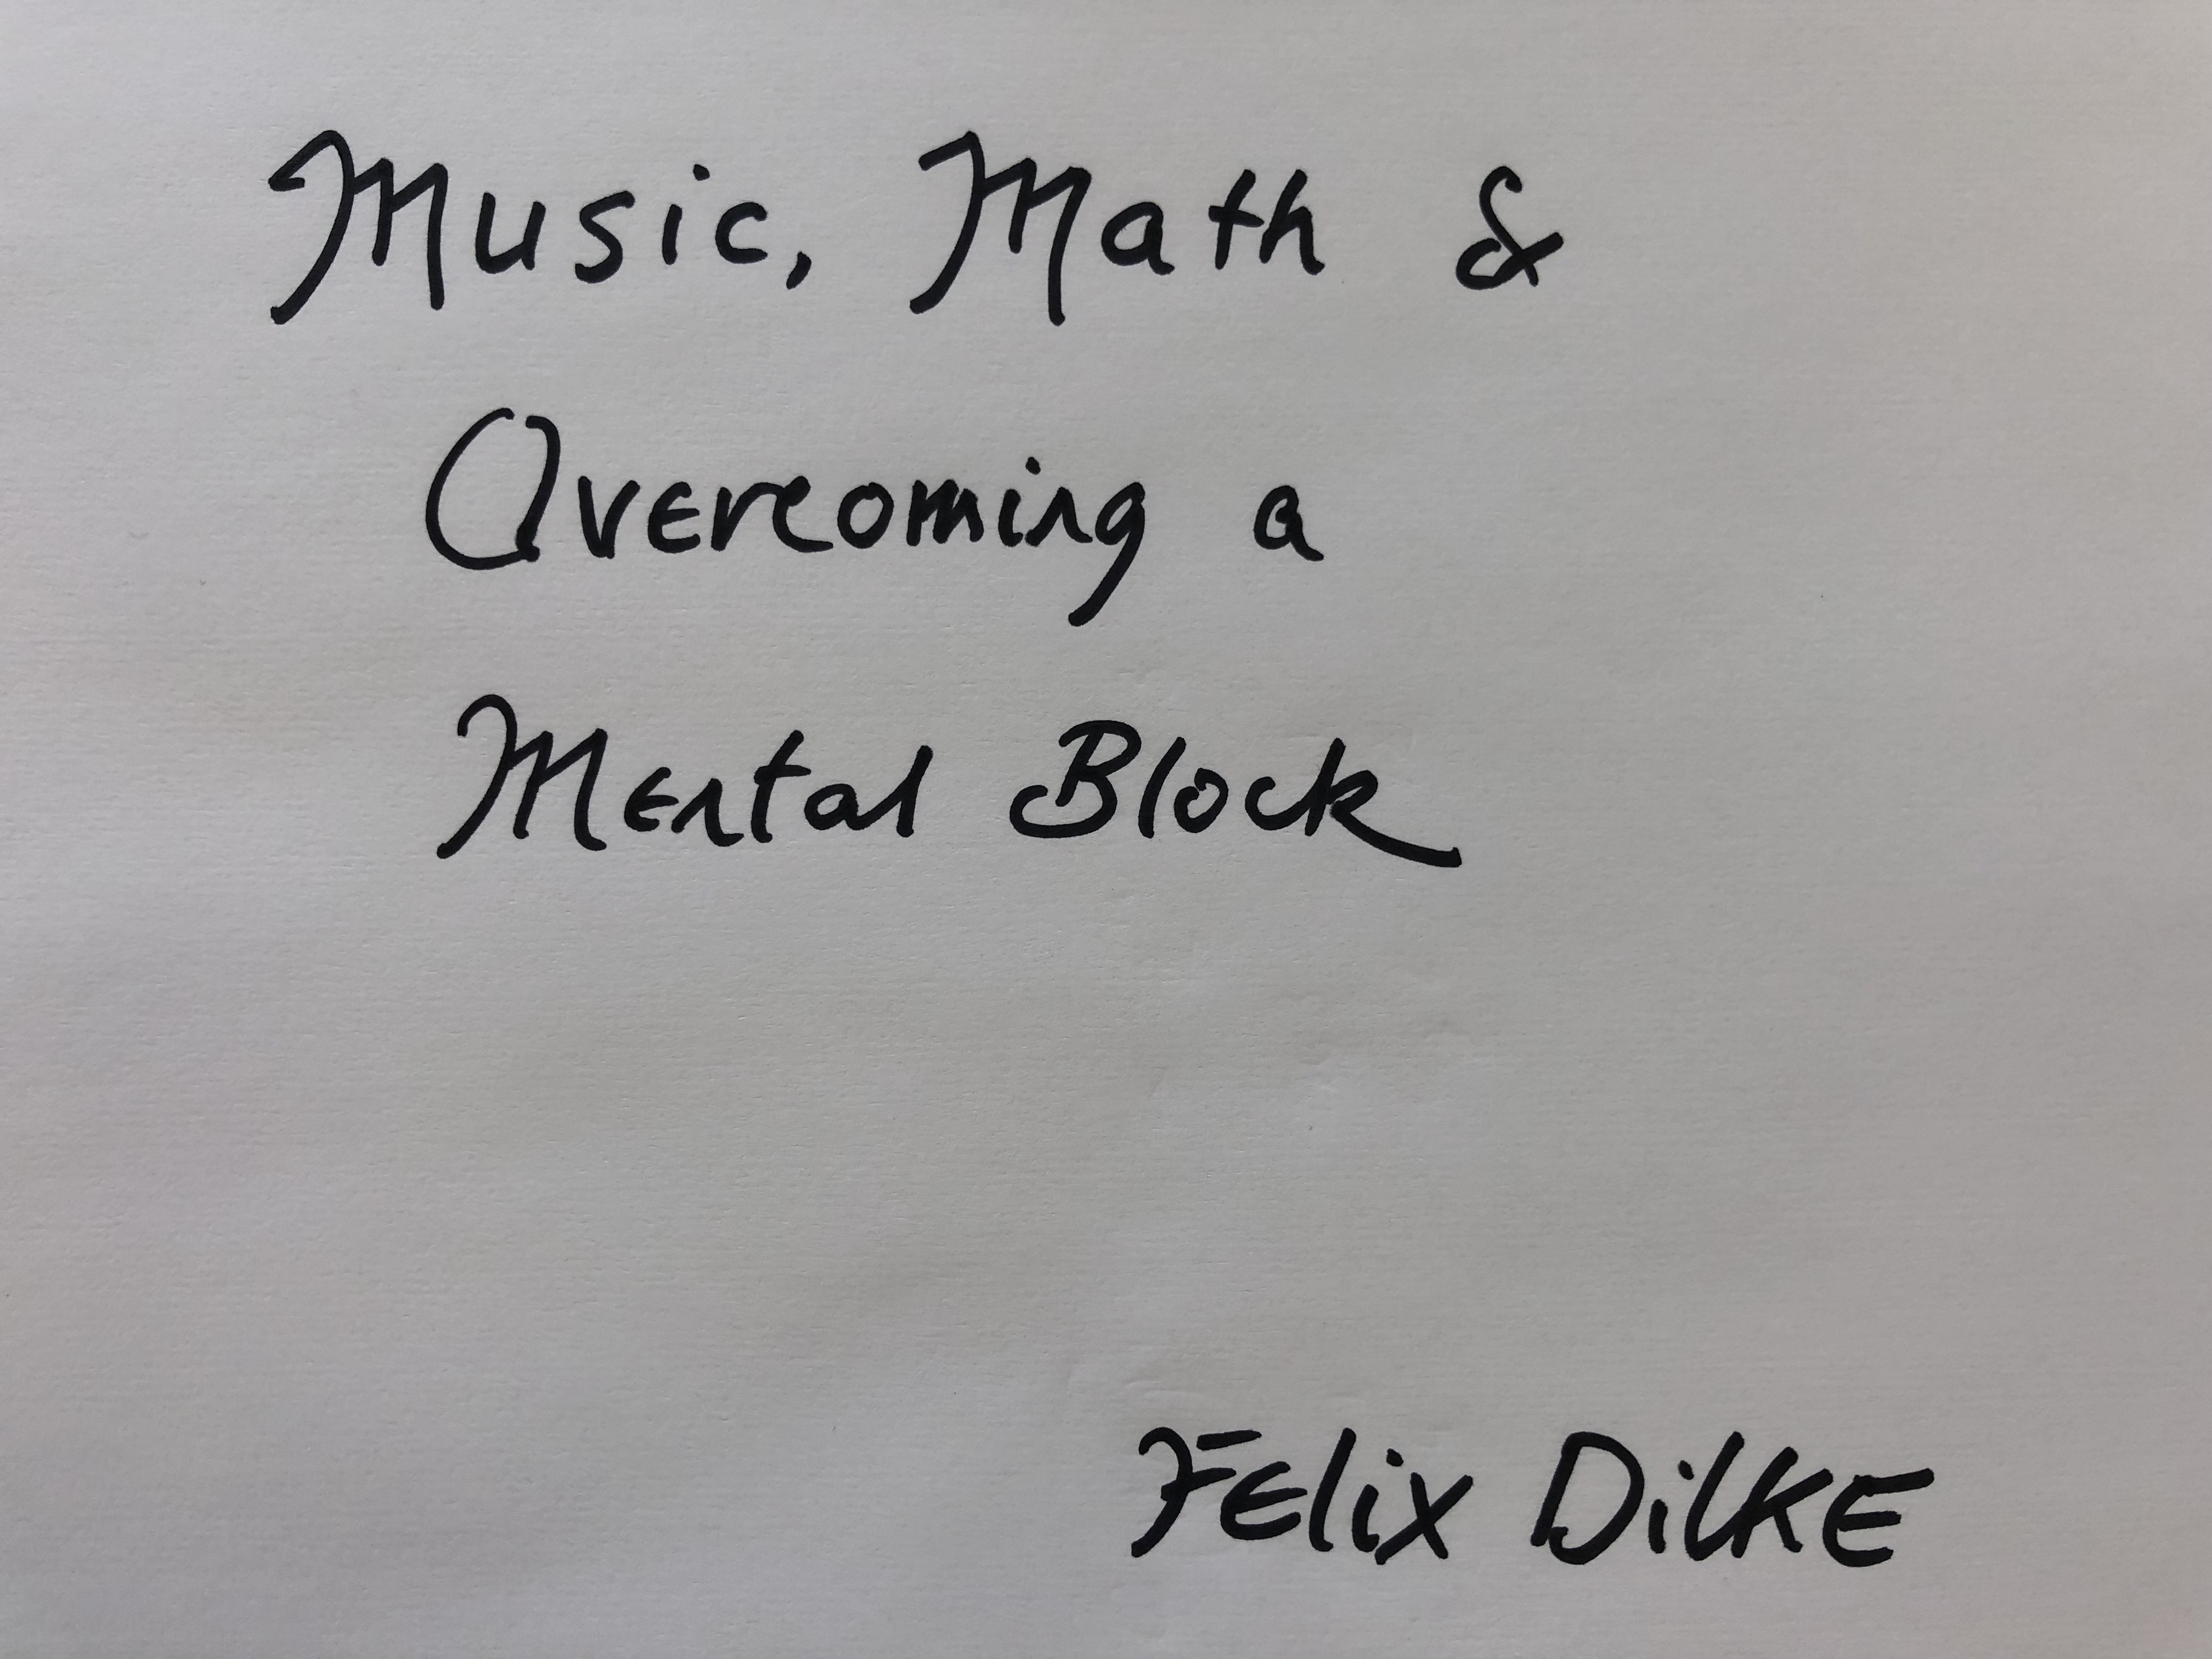
\includegraphics{a}|
% will pick up |a.eps| or |a.wmf|.
% This list can be reset with |\DeclareGraphicsExtensions|.
% Other extensions not in the list may be used explicitly, eg
% |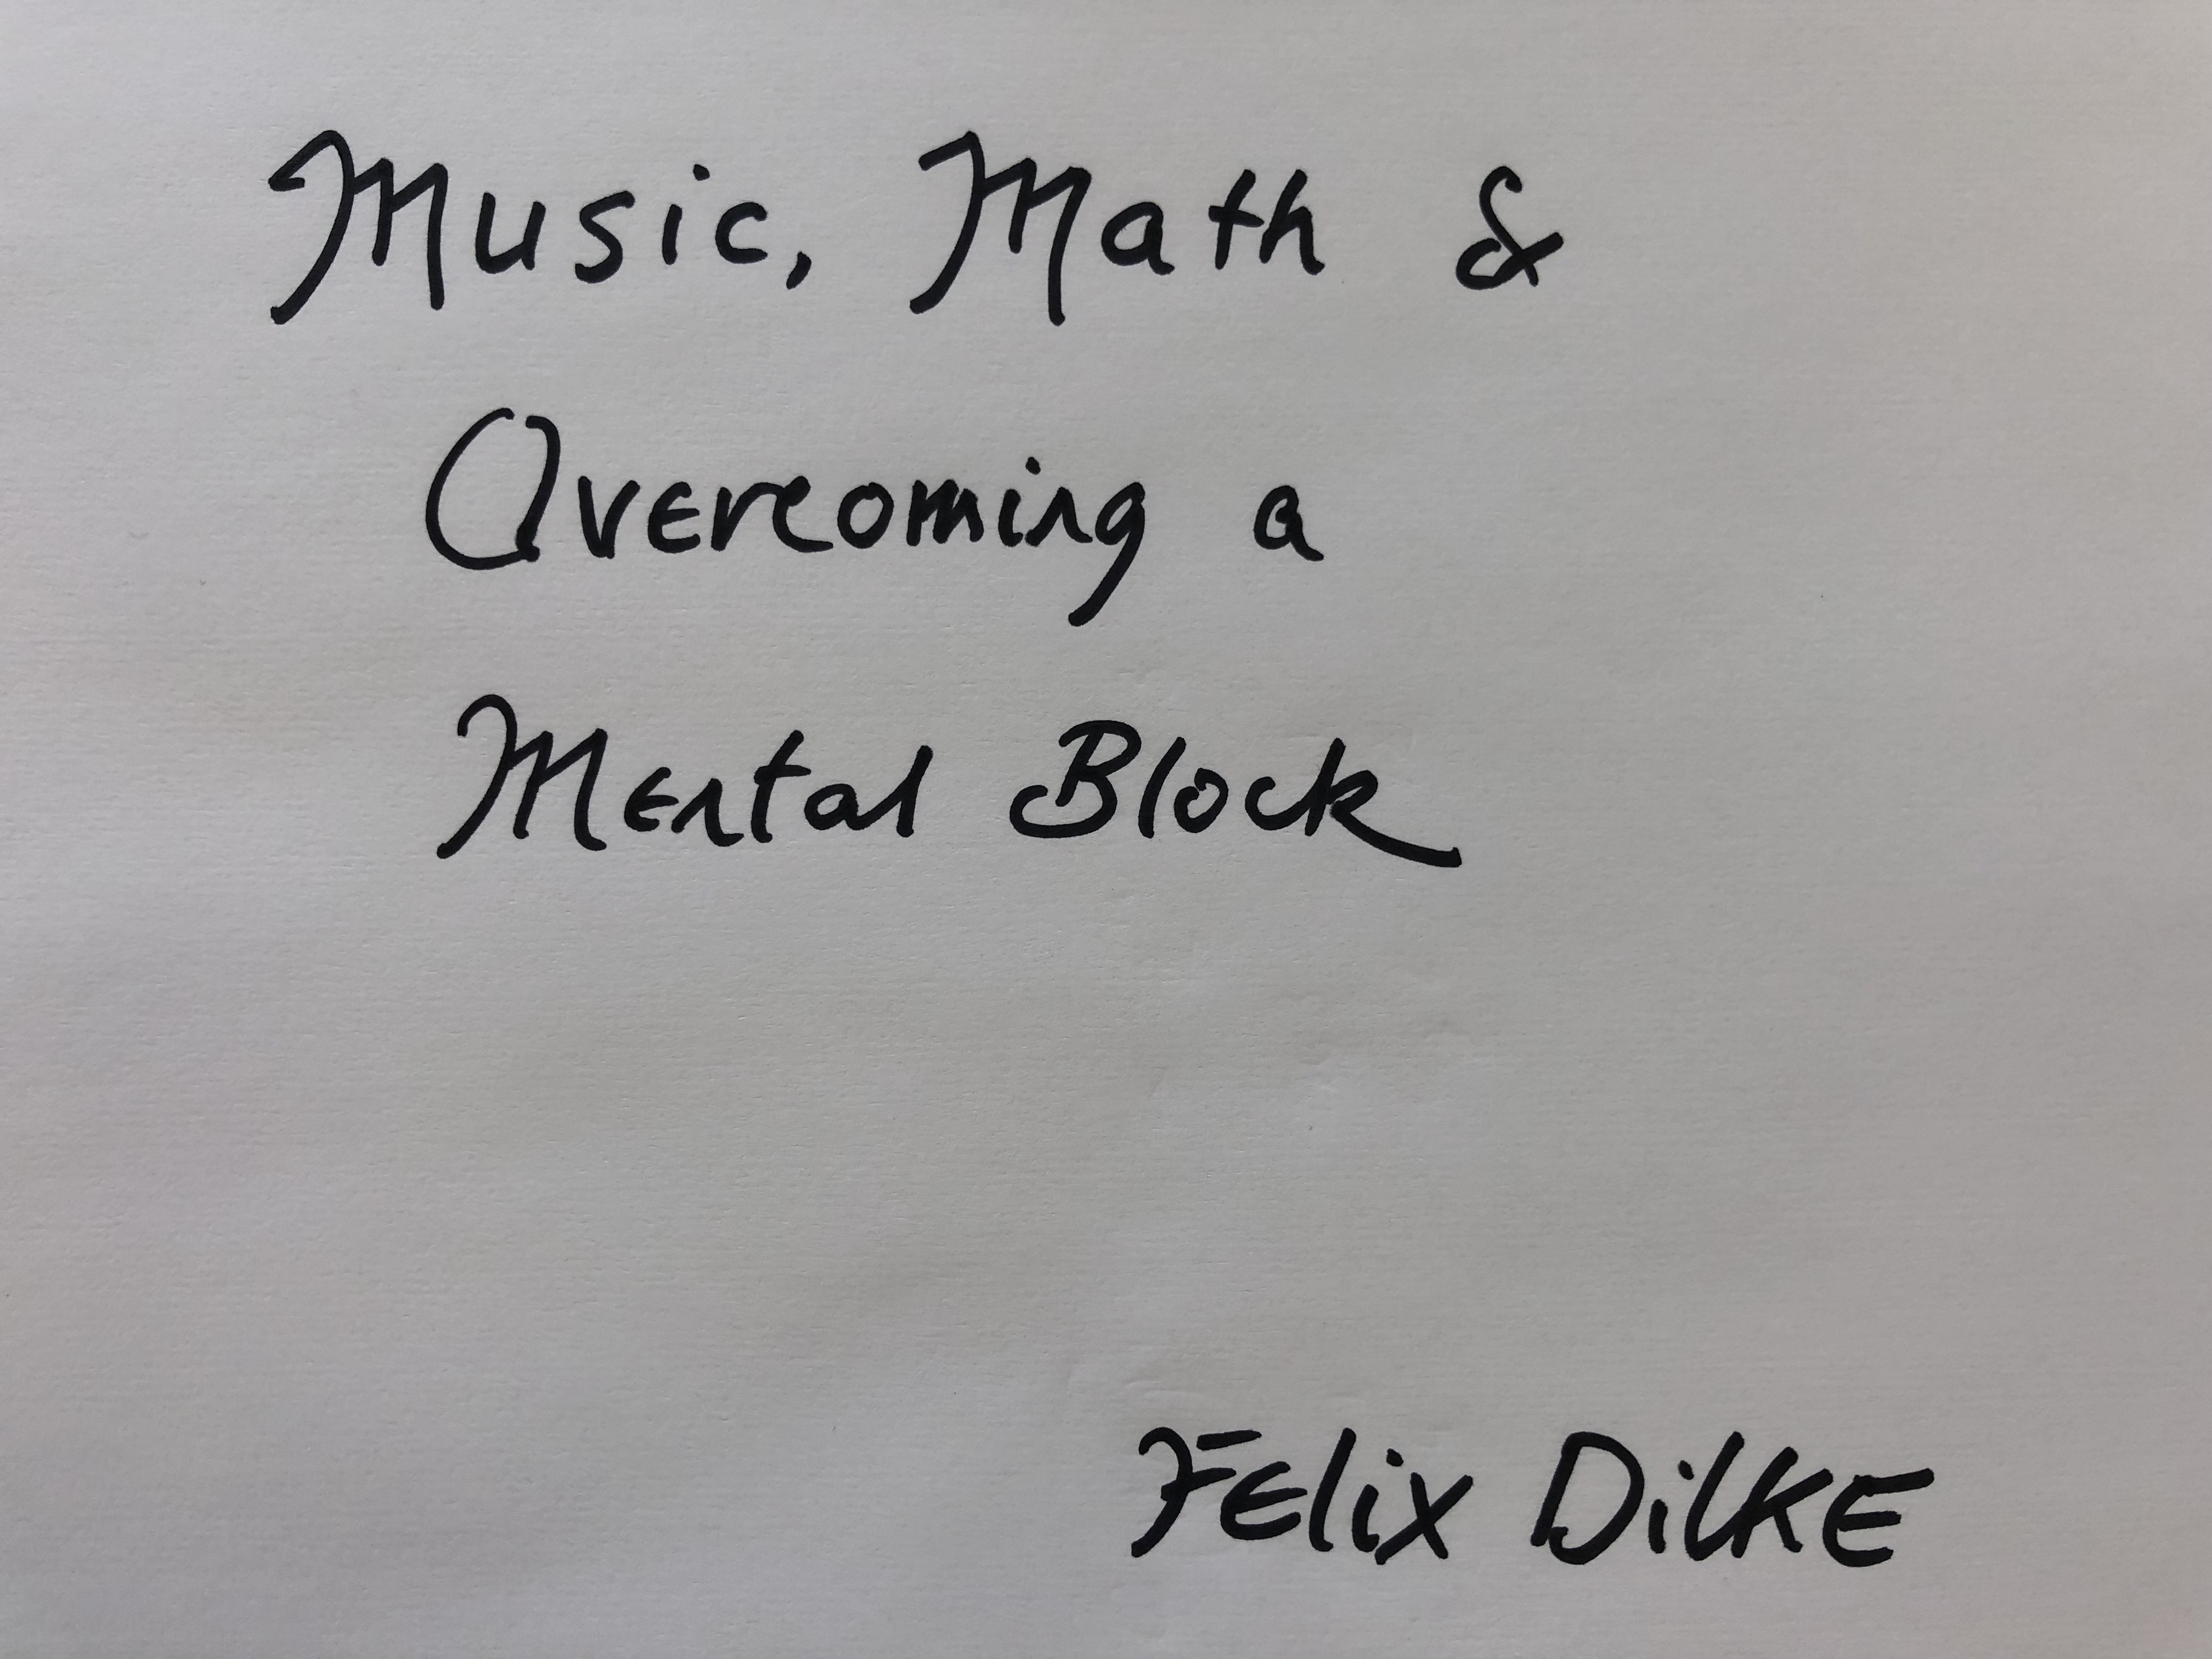
\includegraphics{a.gif}| should work as long as dviwin has access
% to a gif filter. If |.gif| is added using |\DeclareGraphicsExtensions|
% then  |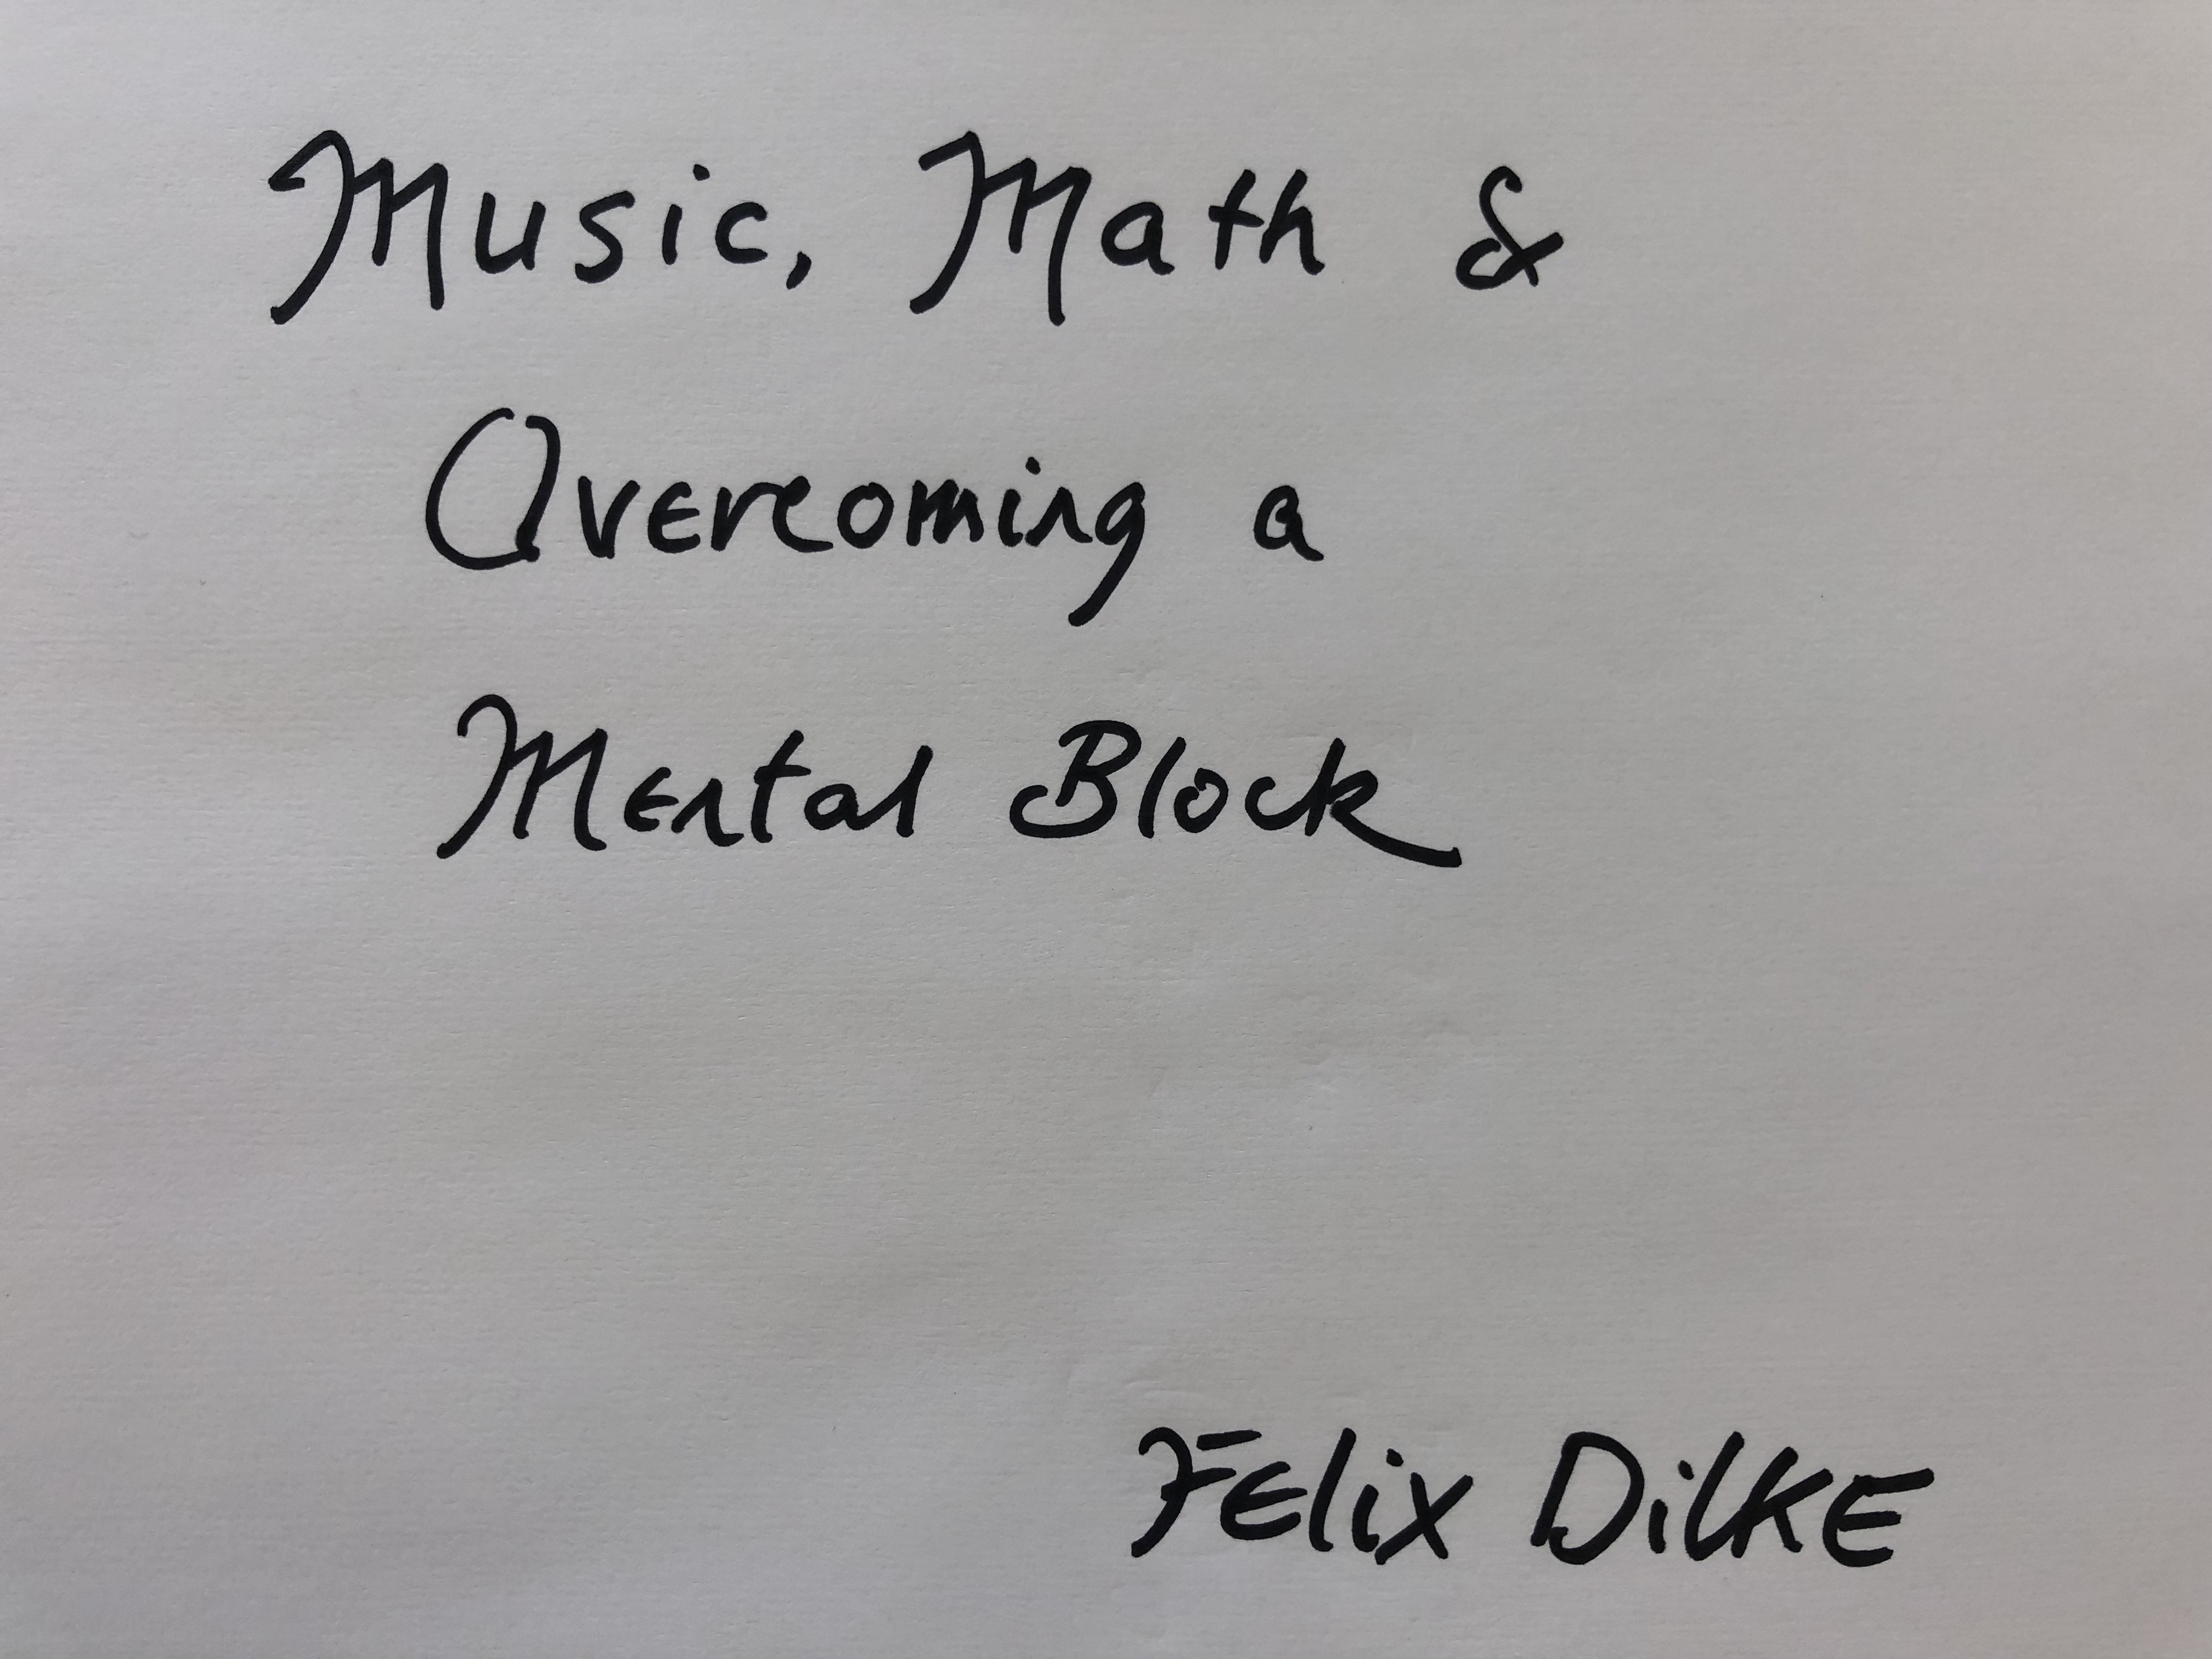
\includegraphics{a}| would also find |a.gif|.
%    \begin{macrocode}
\def\Gin@extensions{.eps,.ps,.wmf,.tif}
%    \end{macrocode}
%
%    \begin{macrocode}
%</dviwin>
%    \end{macrocode}
%
% \section{ln}
% A \LaTeXe\ graphics driver file for B Hamilton Kelly's ln03 driver.
% Untested, but based on the graphics macros distributed with the
% driver.
%    \begin{macrocode}
%<*ln>
%    \end{macrocode}
% \subsection{Graphic file inclusion}
%    \begin{macrocode}
\def\Ginclude@sixel#1{\special{ln03:sixel #1}}
%</ln>
%    \end{macrocode}
%
% \section{truetex}
% A \LaTeXe\ graphics driver file for Kinch `truetex' driver.
%    \begin{macrocode}
%<*truetex>
%    \end{macrocode}
%
% \subsection{Colour}
% Uses the `color4' colour code.
%
% \subsection{Graphic file inclusion}
%
%  EPS File inclusion: DVIPS style.
%    \begin{macrocode}
\def\Ginclude@eps#1{%
 \message{<#1>}%
  \bgroup
  \def\@tempa{!}%
  \dimen@\Gin@req@width
  \dimen@ii.1bp%
  \divide\dimen@\dimen@ii
  \@tempdima\Gin@req@height
  \divide\@tempdima\dimen@ii
    \special{PSfile="#1"\space
      llx=\Gin@llx\space
      lly=\Gin@lly\space
      urx=\Gin@urx\space
      ury=\Gin@ury\space
      \ifx\Gin@scalex\@tempa\else rwi=\number\dimen@\space\fi
      \ifx\Gin@scaley\@tempa\else rhi=\number\@tempdima\space\fi
      \ifGin@clip clip\fi}%
  \egroup}
%    \end{macrocode}
%
% bmp File Inclusion.
%    \begin{macrocode}
\def\Ginclude@bmp#1{%
 \message{<#1>}%
 \special{bmpfile #1}}
%    \end{macrocode}
%
% tif(f) File inclusion
%    \begin{macrocode}
\def\Ginclude@tiff#1{%
 \message{<#1>}%
 \special{tifffile #1}}
%    \end{macrocode}
%
% \subsection{Literal PostScript}
% This is not supported, so uses `nops' code.
%
% \subsection{Default Rules}
% Support (e)ps, tif and bmp, default to eps.
%    \begin{macrocode}
\def\Gin@extensions{.eps,.ps}
\@namedef{Gin@rule@.ps}#1{{eps}{.ps}{#1}}
\@namedef{Gin@rule@.eps}#1{{eps}{.eps}{#1}}
\@namedef{Gin@rule@.tif}#1{{tiff}{}{#1}}
\@namedef{Gin@rule@.bmp}#1{{bmp}{}{#1}}
%    \end{macrocode}
%
%    \begin{macrocode}
\@namedef{Gin@rule@*}#1{{eps}{\Gin@ext}{#1}}
%    \end{macrocode}
%
%    \begin{macrocode}
%</truetex>
%    \end{macrocode}
%
% \section{tcidvi}
% A \LaTeXe\ graphics driver file for Scientific Word/Workplace.
% Actually for the Kinch truetex driver, augmented with extra
% |\special| handling with the DLL supplied with SW.
%    \begin{macrocode}
%<*tcidvi>
%    \end{macrocode}
%
% \subsection{Colour}
% Uses the `color4' colour code.
%
% The above colours are handled by the Kinch-supplied dll
% The TCI dll adds support for |\colorbox|, but only grey scale
% The code below accepts any color model, but only the red
%  component is used.
%    \begin{macrocode}
\AtBeginDocument{\def\color@block#1#2#3{%
  {\rlap{\ifcolors@
      \@defaultunits\count@\current@color\@nnil
      \dimen@\count@\p@
      \divide\dimen@\@cclv
      \dimen@ii#2%
      \advance\dimen@ii#3%
      \lower#3\hbox{%
      \special{language "Scientific Word";%
               type "greybox";%
               greyscale \strip@pt\dimen@;%
               height \the\dimen@ii;%
               width \the#1;%
               depth 0pt;}}%
           \fi}}}}
%    \end{macrocode}
%
% \subsection{Graphic file inclusion}
%
%  EPS File inclusion.
%    \begin{macrocode}
\def\Ginclude@eps#1{%
 \message{<#1>}%
 \raise\Gin@req@height\hbox{%
%    \end{macrocode}
%
% If the bounding box has been changed by a trim or viewport
% key then need to calculate the crop ratios based on the original
% bb coordinates. (This assumes that clip key is also used).
%    \begin{macrocode}
  \ifx\Gin@ollx\@undefined
  \else
    \@tempdimb \Gin@ourx bp%
    \advance\@tempdimb-\Gin@ollx bp%
    \@tempdima\Gin@llx bp%
    \advance\@tempdima-\Gin@ollx bp%
    \Gscale@div\TCI@cropleft\@tempdima\@tempdimb
    \@tempdima\Gin@urx bp%
    \advance\@tempdima-\Gin@ollx bp%
    \Gscale@div\TCI@cropright\@tempdima\@tempdimb
    \@tempdimb \Gin@oury bp%
    \advance\@tempdimb-\Gin@olly bp%
    \@tempdima\Gin@lly bp%
    \advance\@tempdima-\Gin@olly bp%
    \Gscale@div\TCI@cropbottom\@tempdima\@tempdimb
    \@tempdima\Gin@ury bp%
    \advance\@tempdima-\Gin@olly bp%
    \Gscale@div\TCI@croptop\@tempdima\@tempdimb
  \fi
%    \end{macrocode}
%
%    \begin{macrocode}
    \special{%
      language \TCI@language;%
      type \TCI@type;%
      valid_file \TCI@validfile;%
      width \the\Gin@req@width;%
      height \the\Gin@req@height;%
      depth 0pt;%
      original-width \the\Gin@nat@width;%
      original-height \the\Gin@nat@height;%
      cropleft "\TCI@cropleft";%
      croptop "\TCI@croptop";%
      cropright "\TCI@cropright";%
      cropbottom "\TCI@cropbottom";%
      filename '#1';%
      \ifx\TCI@temp\@empty\else tempfilename \TCI@temp;\fi
      }}}
%    \end{macrocode}
%
% Default values so documents produced elsewhere should work
%    \begin{macrocode}
\def\TCI@language{"Scientific Word"}
\def\TCI@type{"GRAPHIC"}
\def\TCI@validfile{'F'}
\def\TCI@cropleft{0}
\def\TCI@croptop{1}
\def\TCI@cropright{1}
\def\TCI@cropbottom{0}
\let\TCI@temp\@empty
%    \end{macrocode}
%
% Non PS Graphic files.
%
% File inclusion macro is always the same. Use a different name though
% as LaTeX thinks it can read eps files for BoundingBox.
%    \begin{macrocode}
\let\Ginclude@bmp\Ginclude@eps
%    \end{macrocode}
%
% \subsection{Literal PostScript}
% This is not supported, so uses `nops' code.
%
% \subsection{Default Rules}
% SW always gives the full name with extension.
% So leave this list empty.
%    \begin{macrocode}
\def\Gin@extensions{}
%    \end{macrocode}
%
% .ps .PS .eps .EPS are (E)PS
% rest are `bmp' which is a catch all type for anything
% that the import filter can handle.
%    \begin{macrocode}
\@namedef{Gin@rule@.ps}#1{{eps}{.ps}{#1}}
\@namedef{Gin@rule@.eps}#1{{eps}{.eps}{#1}}
\@namedef{Gin@rule@.PS}#1{{eps}{.PS}{#1}}
\@namedef{Gin@rule@.EPS}#1{{eps}{.EPS}{#1}}
%    \end{macrocode}
%
%    \begin{macrocode}
\@namedef{Gin@rule@*}#1{{bmp}{\Gin@ext}{#1}}
%    \end{macrocode}
%
%    \begin{macrocode}
%</tcidvi>
%    \end{macrocode}
%
% \section{Literal Postscript}
% Most drivers writing to PostScript allow some form of `literal'
% PostScript |\special| that inserts code into the final PostScript
% output. However Non-PS drivers can not support this (and some PS
% one's can't either). The code here makes all these commands no ops.
% Individual driver sections may define the commands to do something
% useful.
%
%    \begin{macrocode}
%<*nops>
%    \end{macrocode}
%
% Raw PostScript code, no save/restore. Coordinate system unspecified.
%    \begin{macrocode}
\def\Gin@PS@raw#1{}
%    \end{macrocode}
%
% PostScript code, to be surrounded by save/restore by the driver.
% Coordinate system standard PostScript, but with origin
% at current (\TeX) position.
%    \begin{macrocode}
\def\Gin@PS@restored#1{}
%    \end{macrocode}
%
% PostScript code to be inserted in the Header section of the final
% PostScript. Must be issued on the first page of a document.
%    \begin{macrocode}
\def\Gin@PS@literal@header#1{}
%    \end{macrocode}
%
% Name of external file, the contents of which are to be inserted in
% the Header section of the final PostScript. Must be issued on the
% first page of a document.
%    \begin{macrocode}
\def\Gin@PS@file@header#1{}
%    \end{macrocode}
%
%    \begin{macrocode}
%</nops>
%    \end{macrocode}
%
% \section{Graphics Inclusion Rules}
%    \begin{macrocode}
%<*psrules>
%    \end{macrocode}
%
%    \begin{macrocode}
\def\Gin@extensions{.eps,.ps}
%    \end{macrocode}
%
%    \begin{macrocode}
\@namedef{Gin@rule@.ps}#1{{eps}{.ps}{#1}}
\@namedef{Gin@rule@.eps}#1{{eps}{.eps}{#1}}
%    \end{macrocode}
%
%    \begin{macrocode}
\@namedef{Gin@rule@*}#1{{eps}{\Gin@ext}{#1}}
%    \end{macrocode}
%
%    \begin{macrocode}
%</psrules>
%<*psrulesZ>
%    \end{macrocode}
%
% \changes{v3.0j}{2014/04/23}
%     {add .mps for metapost generated postscript to match pdftex graphics/4050}
%    \begin{macrocode}
\def\Gin@extensions{.eps,.ps,.eps.gz,.ps.gz,.eps.Z,.mps}
%    \end{macrocode}
%
% \changes{v3.0k}{2015/12/30}
%     {compressed files don't require gunzip for dvips/xdvi}
%    \begin{macrocode}
\@namedef{Gin@rule@.ps}#1{{eps}{.ps}{#1}}
\@namedef{Gin@rule@.eps}#1{{eps}{.eps}{#1}}
\@namedef{Gin@rule@.mps}#1{{eps}{.mps}{#1}}
\@namedef{Gin@rule@.pz}#1{{eps}{.bb}{#1}}
\@namedef{Gin@rule@.eps.Z}#1{{eps}{.eps.bb}{#1}}
\@namedef{Gin@rule@.ps.Z}#1{{eps}{.ps.bb}{#1}}
\@namedef{Gin@rule@.ps.gz}#1{{eps}{.ps.bb}{#1}}
\@namedef{Gin@rule@.eps.gz}#1{{eps}{.eps.bb}{#1}}
%    \end{macrocode}
%
%    \begin{macrocode}
\@namedef{Gin@rule@*}#1{{eps}{\Gin@ext}{#1}}
%    \end{macrocode}
%
%    \begin{macrocode}
%</psrulesZ>
%<*dosrules>
%    \end{macrocode}
%
%    \begin{macrocode}
%<!psrulesZ>\def\Gin@extensions{.eps,.ps,.pcx,.bmp}
%    \end{macrocode}
%
%    \begin{macrocode}
\@namedef{Gin@rule@.pcx}#1{{bmp}{}{#1}}
\@namedef{Gin@rule@.bmp}#1{{bmp}{}{#1}}
\@namedef{Gin@rule@.msp}#1{{bmp}{}{#1}}
%    \end{macrocode}
%
%    \begin{macrocode}
%</dosrules>
%<*macrules>
%\def\Gin@extensions{{},.ps,.eps,.pict}
%\@namedef{Gin@rule@.ps}#1{{eps}{.ps}{#1}}
%\@namedef{Gin@rule@.eps}#1{{eps}{.eps}{#1}}
\@namedef{Gin@rule@.pict}#1{{pict}{}{#1}}
\@namedef{Gin@rule@.pntg}#1{{pntg}{}{#1}}
%\@namedef{Gin@rule@}#1{{pict}{\relax}{#1}}
%</macrules>
%<*tiffrules>
\@namedef{Gin@rule@.tif}#1{{tiff}{}{#1}}
%</tiffrules>
%    \end{macrocode}
%
% \Finale
%
